\documentclass[11pt]{article}
% The report's page layout. The fonts, colours and diagram styles are in figure-style.tex.

% Fonts, colours, TikZ styles and macros that every diagram and plot uses.
% Loaded by style.tex (the report) and by make-diagrams.py (one file per diagram).

\usepackage{amsmath}
\usepackage{newtxmath}
% Tectonic runs XeTeX without system fonts, so load the TeX Gyre fonts by file name:
% Termes (a Times) for the text, Heros (a Helvetica) for headings and labels.
\usepackage{fontspec}
\setmainfont{texgyretermes}[Extension=.otf, UprightFont=*-regular, BoldFont=*-bold,
  ItalicFont=*-italic, BoldItalicFont=*-bolditalic]
\setsansfont{texgyreheros}[Extension=.otf, UprightFont=*-regular, BoldFont=*-bold,
  ItalicFont=*-italic, BoldItalicFont=*-bolditalic, Scale=0.92]

\usepackage{xcolor}
\usepackage{tikz}
\usepackage{pgfplots}
\pgfplotsset{compat=1.18}
\usetikzlibrary{arrows.meta, positioning, fit, calc, shapes.geometric, backgrounds,
  decorations.pathreplacing}

% One palette for every figure: a layer has one colour everywhere.
\definecolor{mcu}{HTML}{E8F1FB}       % motion: the Arduino, the belt, the arm
\definecolor{mcuedge}{HTML}{2F6DB5}
\definecolor{host}{HTML}{EAF6EC}      % the PC and its program
\definecolor{hostedge}{HTML}{2E7D32}
\definecolor{ui}{HTML}{FFF4E0}        % messages: the serial link and its commands
\definecolor{uiedge}{HTML}{C77700}
\definecolor{vis}{HTML}{F3ECFA}       % vision: the webcam and OpenCV
\definecolor{visedge}{HTML}{7B3FA8}
\definecolor{hw}{HTML}{F1F1F1}        % body and other hardware
\definecolor{hwedge}{HTML}{555555}
\definecolor{warn}{HTML}{FDECEC}
\definecolor{warnedge}{HTML}{B3261E}

\tikzset{
  >={Stealth[length=2mm]},
  box/.style={draw, rounded corners=2pt, align=center, font=\footnotesize,
              minimum height=7mm, inner sep=3pt},
  mcubox/.style={box, fill=mcu, draw=mcuedge},
  hostbox/.style={box, fill=host, draw=hostedge},
  uibox/.style={box, fill=ui, draw=uiedge},
  hwbox/.style={box, fill=hw, draw=hwedge},
  visbox/.style={box, fill=vis, draw=visedge},
  warnbox/.style={box, fill=warn, draw=warnedge},
  group/.style={draw, dashed, rounded corners=3pt, inner sep=6pt},
  grouplabel/.style={font=\scriptsize\itshape, anchor=north west},
  flow/.style={->, thick},
  dataflow/.style={->, thick, densely dashed},
  lbl/.style={font=\scriptsize, midway, fill=white, inner sep=1pt},
}

% A file, function or code name, typeset as written (underscores included).
\newcommand{\topic}[1]{\texttt{\detokenize{#1}}}


% --- Page and type: one column, 11 pt, room to breathe -----------------------
\usepackage[a4paper, margin=25mm, headheight=14pt]{geometry}
\usepackage[final]{microtype}
\usepackage{setspace}
\setstretch{1.15}
\setlength{\parindent}{0pt}
\setlength{\parskip}{0.7\baselineskip}
\setlength{\emergencystretch}{2em}   % room for long code names without overfull lines
\usepackage{enumitem}
\setlist{itemsep=2pt, topsep=4pt}

% --- Colour accents ------------------------------------------------------------
\definecolor{accent}{HTML}{1F5FA8}     % headings, links, the title band
\definecolor{accentsoft}{HTML}{EAF2FB}
\definecolor{ink}{HTML}{22262B}
\definecolor{muted}{HTML}{5F6670}
\color{ink}

\usepackage[font={small,sf}, labelfont={bf,color=accent}, margin=8mm, skip=6pt,
  justification=raggedright, singlelinecheck=true]{caption}
% Let figures share pages with text instead of sitting alone on float pages
\renewcommand{\topfraction}{0.9}
\renewcommand{\bottomfraction}{0.8}
\renewcommand{\textfraction}{0.07}
\renewcommand{\floatpagefraction}{0.85}
\setcounter{topnumber}{3}
\setcounter{totalnumber}{4}
\usepackage[section]{placeins}   % keep each section's floats in that section
\usepackage{needspace}           % \Needspace{n\baselineskip} keeps a heading off the page foot
\usepackage{titlesec}
\usepackage[most]{tcolorbox}

\usepackage{fancyhdr}
\pagestyle{fancy}
\fancyhf{}
\fancyhead[L]{\small\sffamily\color{muted} ConveySort-Arm: design and prototype}
\fancyhead[R]{\small\sffamily\color{muted} Technical report, v1.0, October 2026}
\fancyfoot[C]{\small\sffamily\color{muted}\thepage}
\renewcommand{\headrulewidth}{0.4pt}
\renewcommand{\headrule}{{\color{accent!40}\hrule height\headrulewidth}}

% Section headings: sans, accent colour, a thin rule under each section
\titleformat{\section}{\Large\sffamily\bfseries\color{accent}}{\thesection}{0.6em}{}[{\color{accent!30}\titlerule[0.6pt]}]
\titleformat{\subsection}{\large\sffamily\bfseries\color{accent!85!black}}{\thesubsection}{0.6em}{}
\titleformat{\paragraph}[runin]{\sffamily\bfseries\color{ink}}{}{}{}[.]
\titlespacing*{\section}{0pt}{1.6\baselineskip}{0.6\baselineskip}
\titlespacing*{\subsection}{0pt}{1.1\baselineskip}{0.3\baselineskip}
\titlespacing*{\paragraph}{0pt}{0.6\baselineskip}{0.6em}

% Status labels, one colour each, used in the results box and the tables
\newcommand{\chip}[2]{\tikz[baseline=(c.base)]\node[fill=#1!15, draw=#1!70!black, text=#1!60!black,
  rounded corners=2pt, inner xsep=3pt, inner ysep=1.2pt, font=\scriptsize\sffamily\bfseries] (c) {#2};}
\newcommand{\onvideo}{\chip{blue}{shown on video}}
\newcommand{\computed}{\chip{violet}{computed from the code}}

% A soft, coloured box for summaries
\newtcolorbox{summarybox}[1]{colback=accentsoft, colframe=accent, boxrule=0.6pt, arc=2pt,
  left=8pt, right=8pt, top=6pt, bottom=6pt, fonttitle=\sffamily\bfseries, title={#1},
  before upper={\setlength{\parskip}{5pt}}}

% --- Content --------------------------------------------------------------------
\usepackage{graphicx}
\usepackage{adjustbox}
\usepackage{booktabs}
\usepackage{array}
\usepackage{tabularx}
\usepackage{colortbl}
\usepackage{url}
\usepackage{cite}
\usepackage[colorlinks, linkcolor=accent, citecolor=accent, urlcolor=accent]{hyperref}

\graphicspath{{../media/}}

% Table headers in a light accent band
\newcommand{\thead}[1]{\cellcolor{accentsoft}\sffamily\bfseries\small #1}

% A diagram at its natural size, shrunk only if it is wider than the text.
\newcommand{\diagram}[1]{\adjustbox{max width=\textwidth}{\input{#1}}}
% A diagram scaled, up or down, to a share of the text width: \diagramw{0.8}{figures/x}
\newcommand{\diagramw}[2]{\adjustbox{width=#1\textwidth}{\input{#2}}}


\begin{document}

% ---------------------------------------------------------------------------
% Title block
\thispagestyle{empty}
\begin{tcolorbox}[colback=accent, colframe=accent, arc=3pt, left=14pt, right=14pt, top=14pt, bottom=12pt]
  \color{white}\sffamily\raggedright
  {\small Technical report \quad$\cdot$\quad Version 1.0 \quad$\cdot$\quad October 2026}\par\vspace{8pt}
  {\LARGE\bfseries ConveySort-Arm: A Low-Cost Vision-Guided Sorting Cell with a Conveyor Belt and a Six-Servo Arm}\par\vspace{6pt}
  {\large Design and Prototype}
\end{tcolorbox}

\vspace{4pt}
{\sffamily\raggedright
\textbf{Jewel Nath}$^{1,2}$, \mbox{\textbf{Shafiul Alam Chowdhury}$^{2}$}\\[2pt]
{\small\color{muted}$^{1}$Independent researcher, Dhaka, Bangladesh\quad $^{2}$RoboAI, Bangladesh}\\
{\small\color{muted}Jewel Nath: ORCID \href{https://orcid.org/0009-0002-6609-6378}{0009-0002-6609-6378}\quad$\cdot$\quad Code: \url{https://github.com/jewel-nath/conveysort-arm}}\\
{\small\color{muted}Licence: \href{https://creativecommons.org/licenses/by/4.0/}{CC BY 4.0}}\par}

\vspace{6pt}
\begin{summarybox}{Abstract}
ConveySort-Arm is a small sorting cell built in 2024 at RoboAI, Bangladesh, from low-cost parts: a conveyor belt turned by a stepper motor, an ultrasonic sensor at the belt's end, a webcam above it, and a six-servo arm beside it. It brings each block to the arm, measures its size from above, and has the arm set it down in the place for that size.

The work is split between a PC and an Arduino Uno. On the PC, a Python program with OpenCV thresholds each camera frame, finds the block's outline, and calls it small, medium or large by its area; once ten more frames agree on the same size, it sends the size to the Arduino over serial. The Arduino runs the belt until the block reaches the sensor, then moves the arm through a fixed 15-step pick-and-place, with a grip and a set-down place for each size.

The cell was built and run in October and November 2024; videos show the belt bringing blocks to the arm, OpenCV sizing them, and the arm picking them up and setting them down. As programmed, one sort takes 35 to 38 seconds. This report describes the build, the electronics, the vision, the control and the timing of the cell, and sets out the lessons and the next steps, the first being to run the arm from the ROS~2 workspace written for it.

\smallskip
{\sffamily\small\textbf{Keywords:} robotic sorting, pick and place, conveyor, computer vision, OpenCV, Arduino, servo arm, low-cost automation.}
\end{summarybox}

% ---------------------------------------------------------------------------
\section{Introduction}

Sorting objects on a conveyor is one of the oldest jobs for robots in industry: a camera or a sensor tells the objects apart, and an arm moves each one to its place. Research on picking has moved on to unknown objects in clutter~\cite{saxena2008grasping,zeng2018pickplace}, but the basic loop, sense, decide, pick and place, is still the core of the task, and still the best way to learn it.

ConveySort-Arm is a small, low-cost version of that loop (Fig.~\ref{fig:hero}). A belt brings each block to an arm; a webcam and OpenCV measure the block; and the arm sets it down in one of three places by its size. It was built at RoboAI from parts available in Bangladesh: hobby servos, a stepper motor, an ultrasonic sensor, an Arduino and a webcam.

\begin{figure}[htbp]
  \centering
  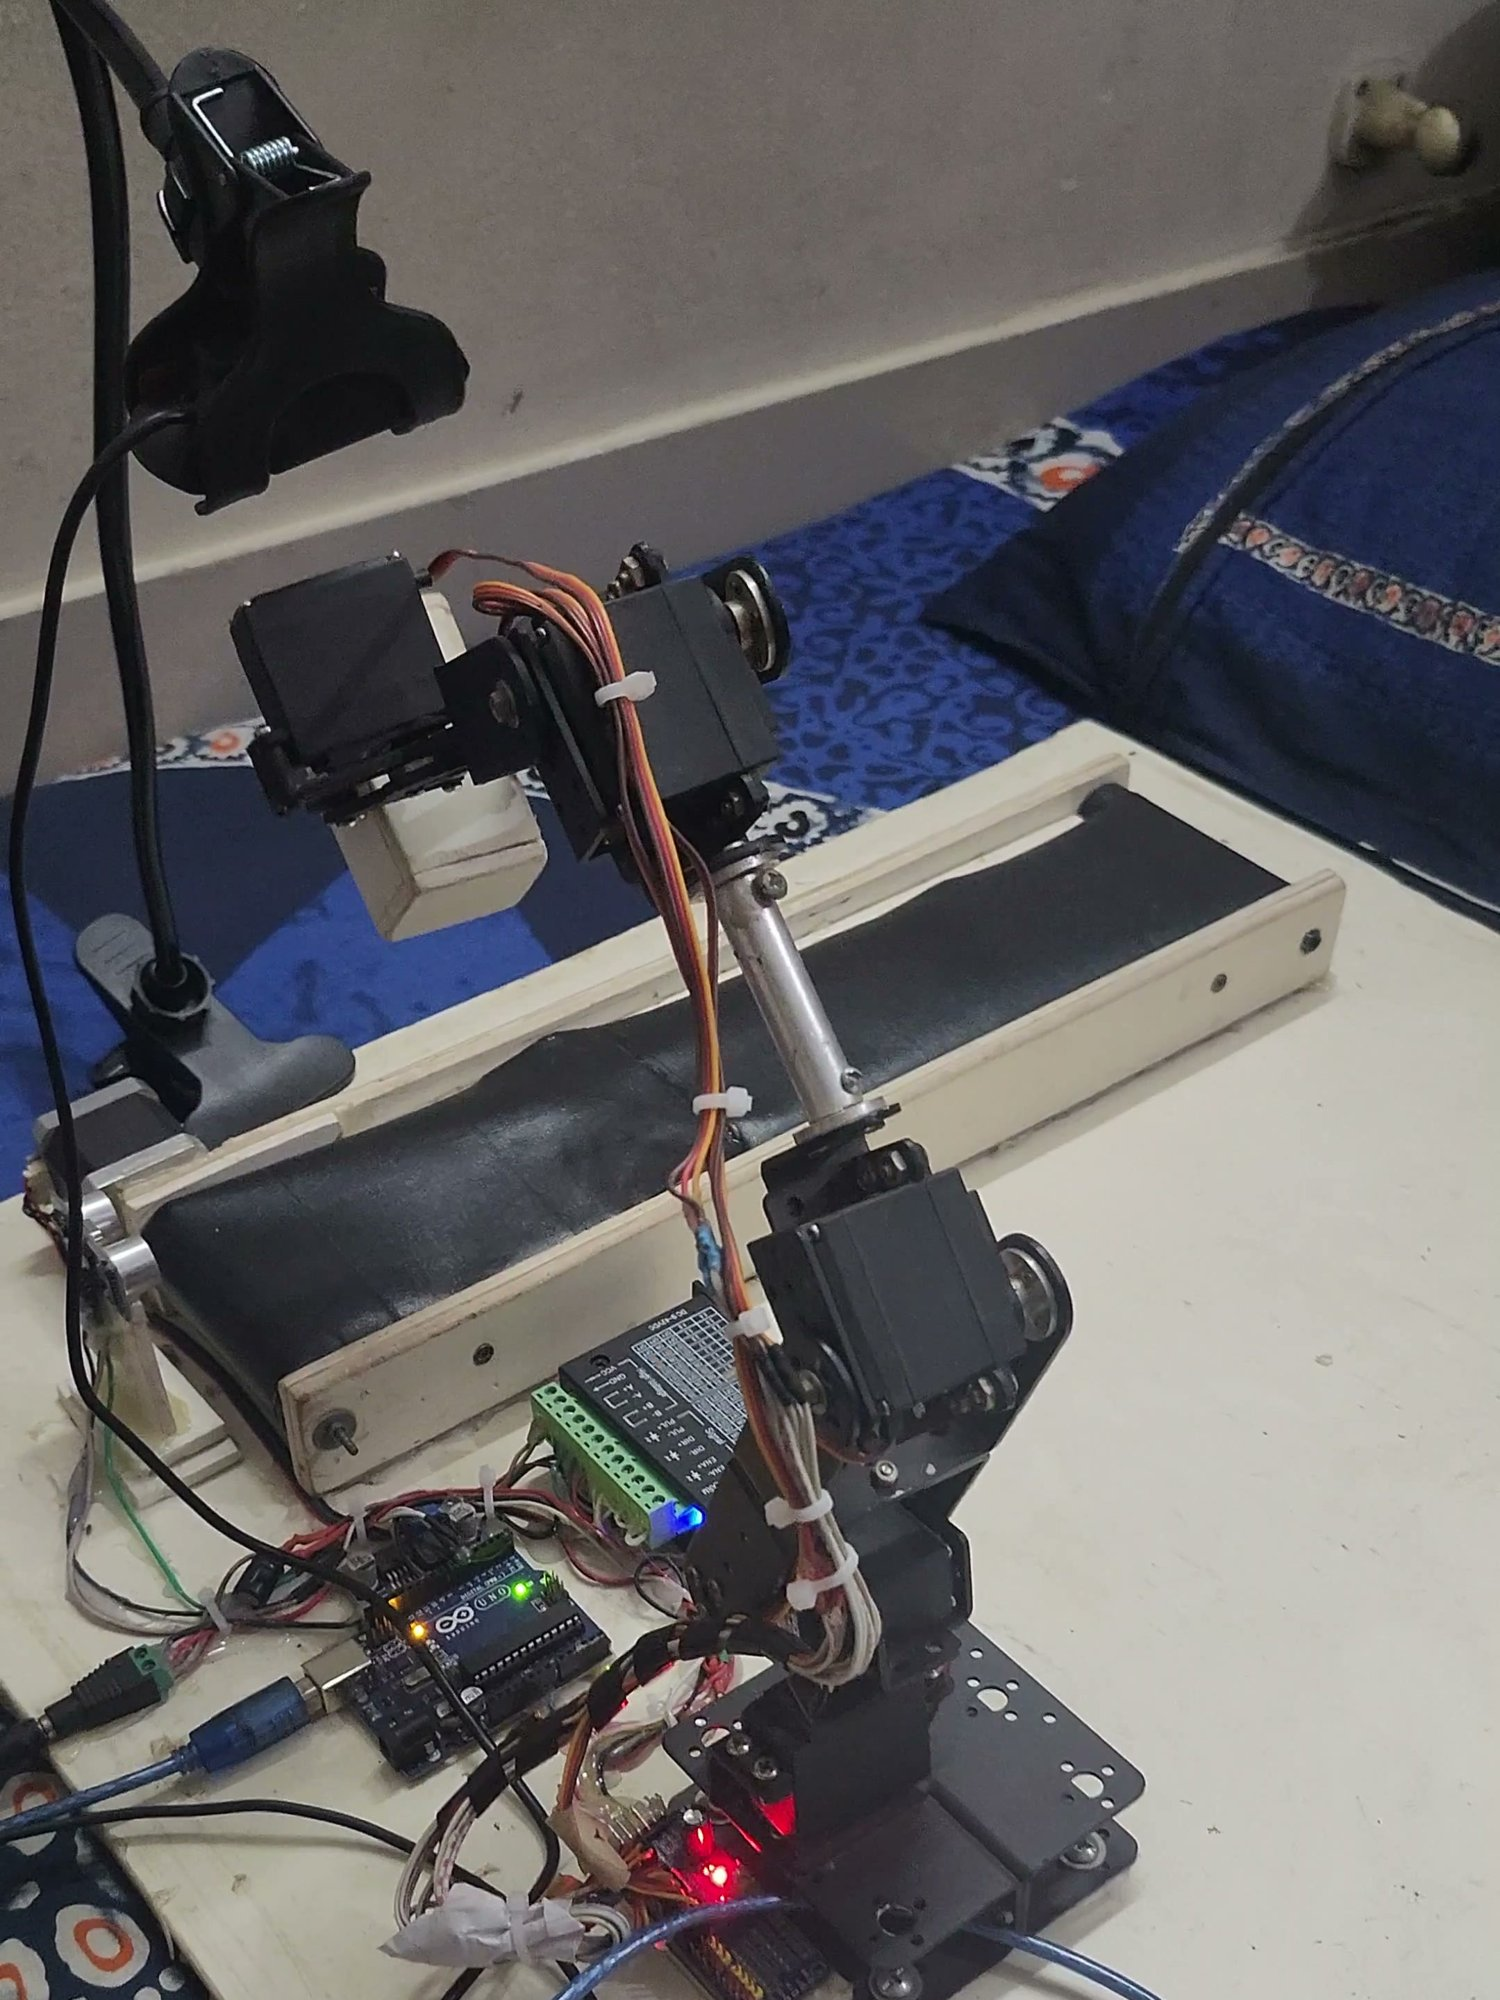
\includegraphics[height=66mm]{conveysort-arm-2024-11-18-arm-lifts-block.jpg}\hspace{4mm}
  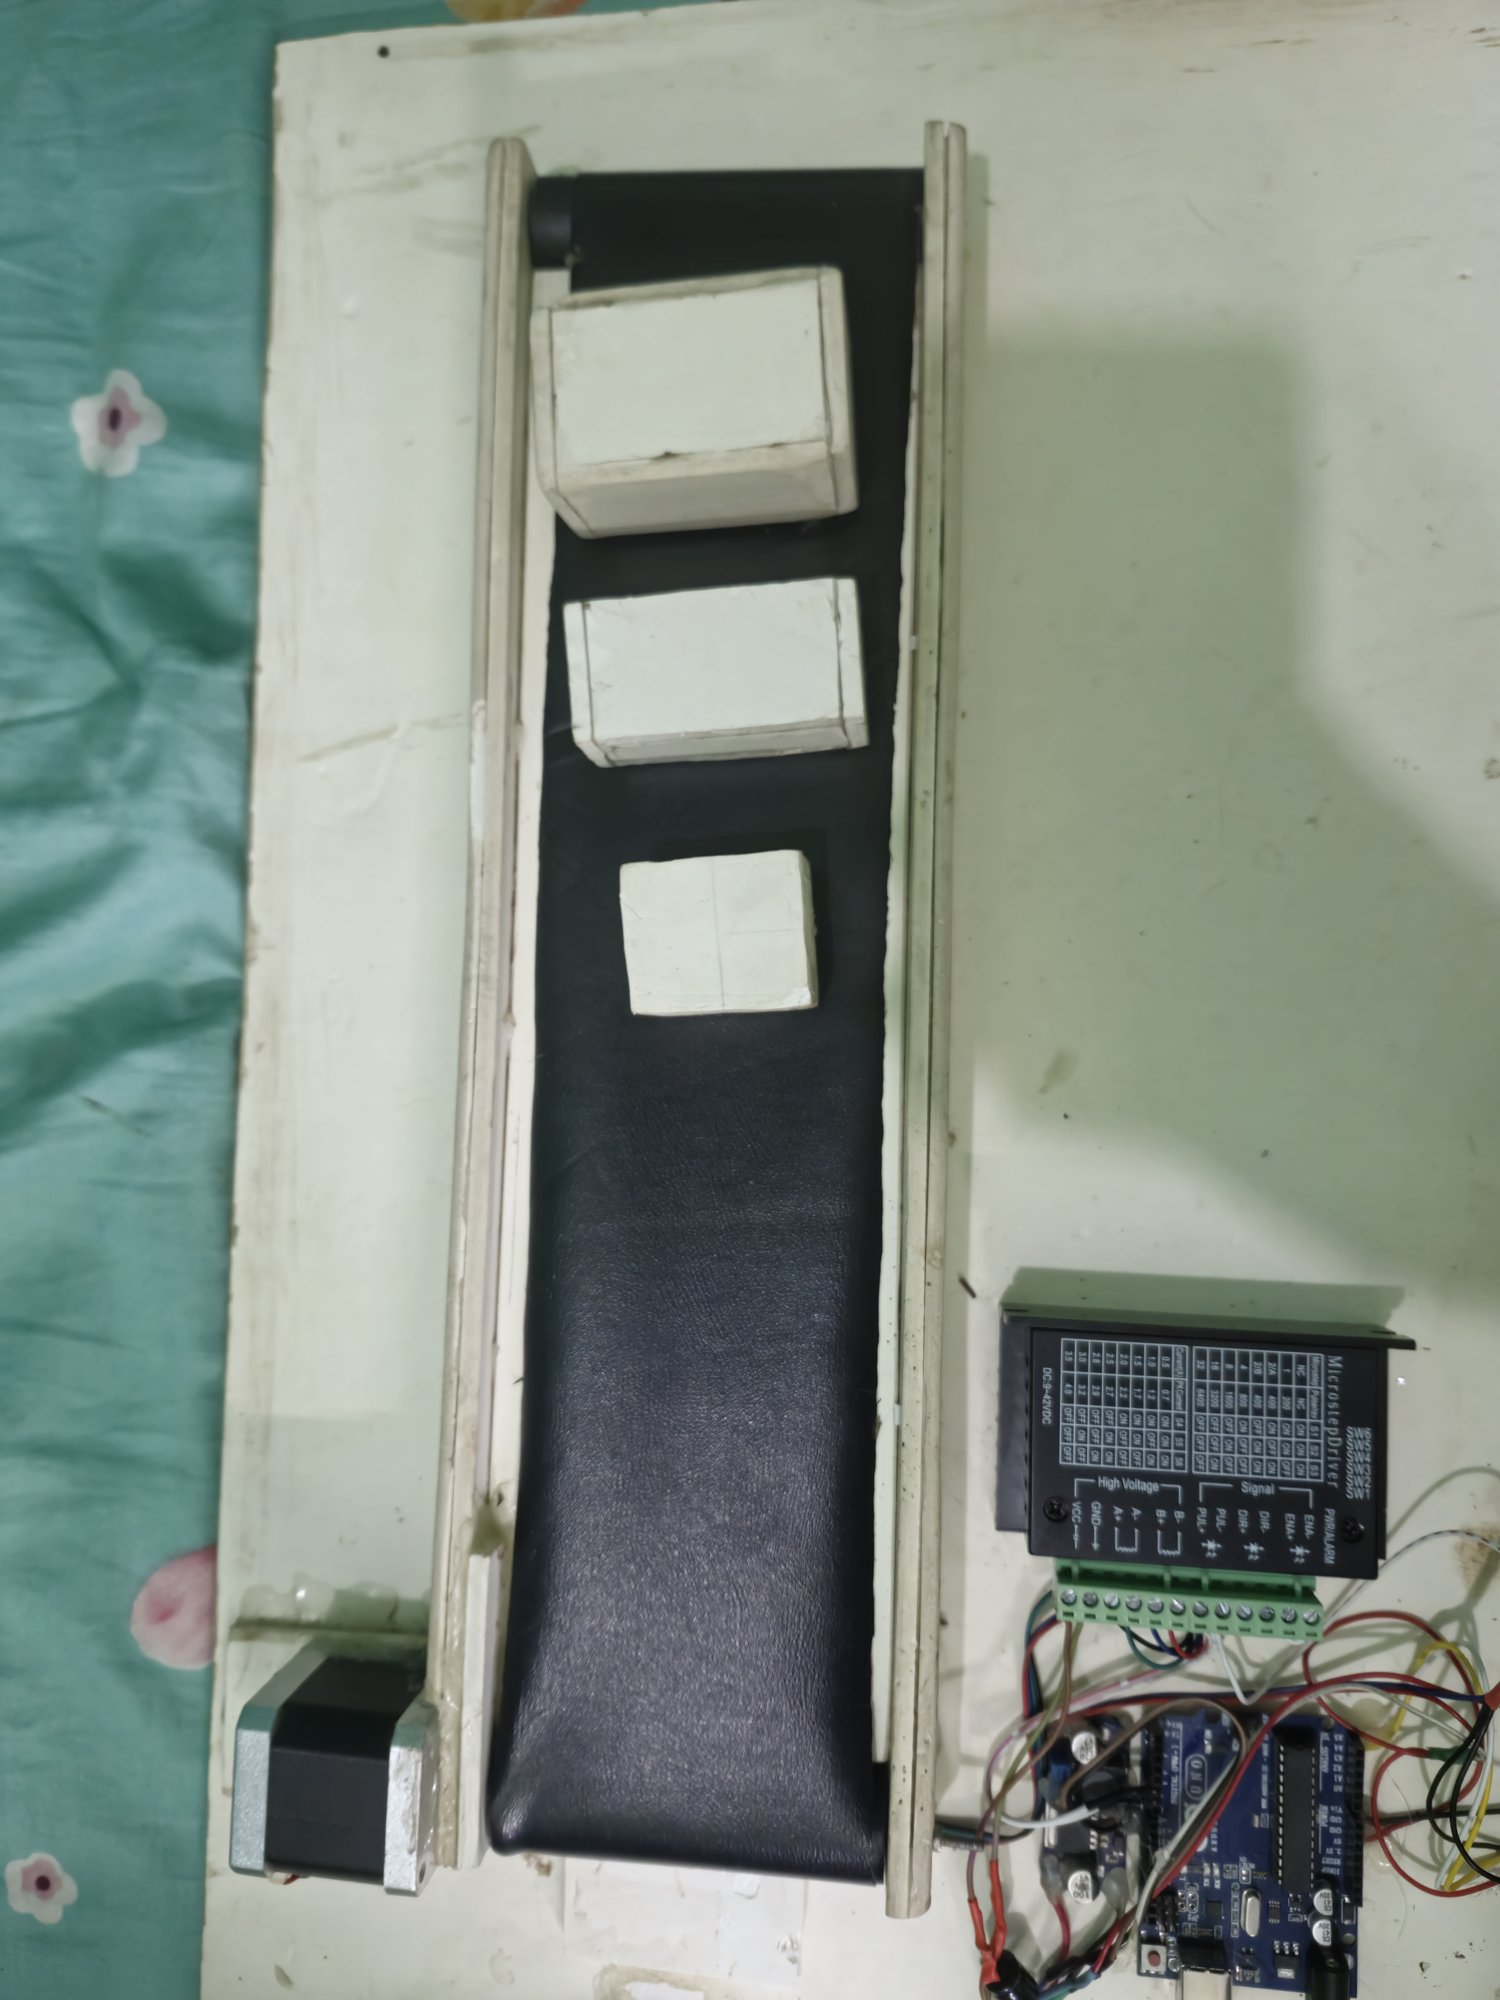
\includegraphics[height=66mm]{conveysort-arm-2024-11-16-conveyor-from-above.jpg}
  \caption{ConveySort-Arm. The arm lifting a block off the belt, the webcam on its clamp above, on 18 November 2024 (left). The conveyor from above with the three test sizes, the stepper motor at the near end, and the driver and the Arduino beside it, on 16 November 2024 (right).}
  \label{fig:hero}
\end{figure}

This report describes the cell as built, and contributes:

\begin{enumerate}
  \item a sorting cell built from low-cost parts: a stepper-driven belt, an ultrasonic stop, a webcam and a six-servo arm (Sections~\ref{sec:build}--\ref{sec:electronics});
  \item size sorting by outline area with OpenCV, steadied over eleven frames in a row before a decision (Section~\ref{sec:vision});
  \item a simple split of the work between a PC, for vision, and an Arduino, for the belt and the arm, joined by a one-character serial protocol (Section~\ref{sec:control});
  \item the timing of a sort, computed from the firmware (Section~\ref{sec:timing});
  \item the behaviours shown on video, and the open source code, under the MIT licence, with its course-derived ROS~2 workspace under Apache~2.0~\cite{conveysortrepo} (Section~\ref{sec:demo}).
\end{enumerate}

\begin{summarybox}{Results at a glance}
\renewcommand{\arraystretch}{1.25}
\small
\begin{tabularx}{\linewidth}{@{}>{\raggedright\arraybackslash}p{0.3\linewidth}X>{\raggedleft\arraybackslash}p{0.24\linewidth}@{}}
  \textbf{\sffamily What the cell does} & \textbf{\sffamily How} & \textbf{\sffamily Evidence} \\
  \midrule
  Brings each block to the arm & the belt runs while the sensor sees a block, and stops it at 7\,cm & \onvideo \\
  Sizes each block from above & OpenCV outlines the block and sizes it by its area & \onvideo \\
  Picks the block up and sets it down & a 15-step sequence on six servos & \onvideo \\
  Puts each size in its own place & a grip and a base angle for each size: 90$^\circ$, 50$^\circ$ or 10$^\circ$ & \chip{gray}{the team's runs} \\
  Sorts one block in 35--38\,s & as programmed, from the command to home & \computed \\
\end{tabularx}
\par\smallskip
{\footnotesize\sffamily The videos were recorded on 11, 16 and 18 November 2024. ``The team's runs'' are the authors' account of their November 2024 tests.}
\end{summarybox}

% ---------------------------------------------------------------------------
\section{Related Work}

\paragraph{Picking with vision} Saxena et al.\ learned grasp points for objects a robot had never seen from images~\cite{saxena2008grasping}, and Zeng et al.\ picked and placed unknown objects from clutter with learned grasp affordances~\cite{zeng2018pickplace}. ConveySort-Arm works in the simpler setting those methods grew from: known objects, one at a time, in a fixed place on a belt, so that a fixed motion can pick each one.

\paragraph{Measuring objects in images} OpenCV~\cite{bradski2000opencv} provides the image operations the cell uses: conversion to grey, blurring, thresholding and outline finding, the last by Suzuki and Abe's border following~\cite{suzuki1985contours}. The block's size is the area inside its outline.

\paragraph{Arms on ROS} ROS~2~\cite{macenski2022ros2} and MoveIt~\cite{coleman2014moveit} are the usual way to model and plan an arm today. The cell's ROS~2 workspace follows Antonio Brandi's course on manipulators~\cite{brandi2023course} (Section~\ref{sec:ros}).

% ---------------------------------------------------------------------------
\section{System Overview}
\label{sec:overview}

Fig.~\ref{fig:overview} shows the cell. A PC reads the webcam and runs the vision program; it sends the Arduino one character, the block's size, over USB serial. The Arduino runs everything that moves: it drives the belt's stepper motor through a TB6600 driver, reads the ultrasonic sensor at the belt's end, and moves the arm's six servos through a PCA9685 servo driver~\cite{pca9685}. It prints a line for each event, which the PC reads back.

\begin{figure}[htbp]
  \centering
  \diagramw{0.98}{figures/fig01-system-overview}
  \caption{System overview. The PC (green) runs the vision (purple) and sends the block's size over the serial link (orange); the Arduino drives the belt and the arm (blue).}
  \label{fig:overview}
\end{figure}

The split keeps each side simple. The PC needs no real-time control, and the Arduino needs no camera: the two agree only on four characters, and the Arduino acts on a size only when the belt has stopped with a block in place.

% ---------------------------------------------------------------------------
\section{Mechanical Build}
\label{sec:build}

The cell grew in two months (Figs.~\ref{fig:build} and~\ref{fig:timeline}). The first version, in early October 2024, put a cloth belt, its stepper motor, the sensor, the Arduino and the arm on one board. By November the belt was a black band in a wooden frame, ending at the ultrasonic sensor, with the arm beside its end. The webcam came last: on a stand above the belt on 16 November, then on a clamp by 18 November.

The arm has six servos: a base, a shoulder, an elbow, a wrist that pitches and rolls, and a gripper. It stands beside the end of the belt, so it can reach the stopped block and three set-down places around its base.

\begin{figure}[htbp]
  \centering
  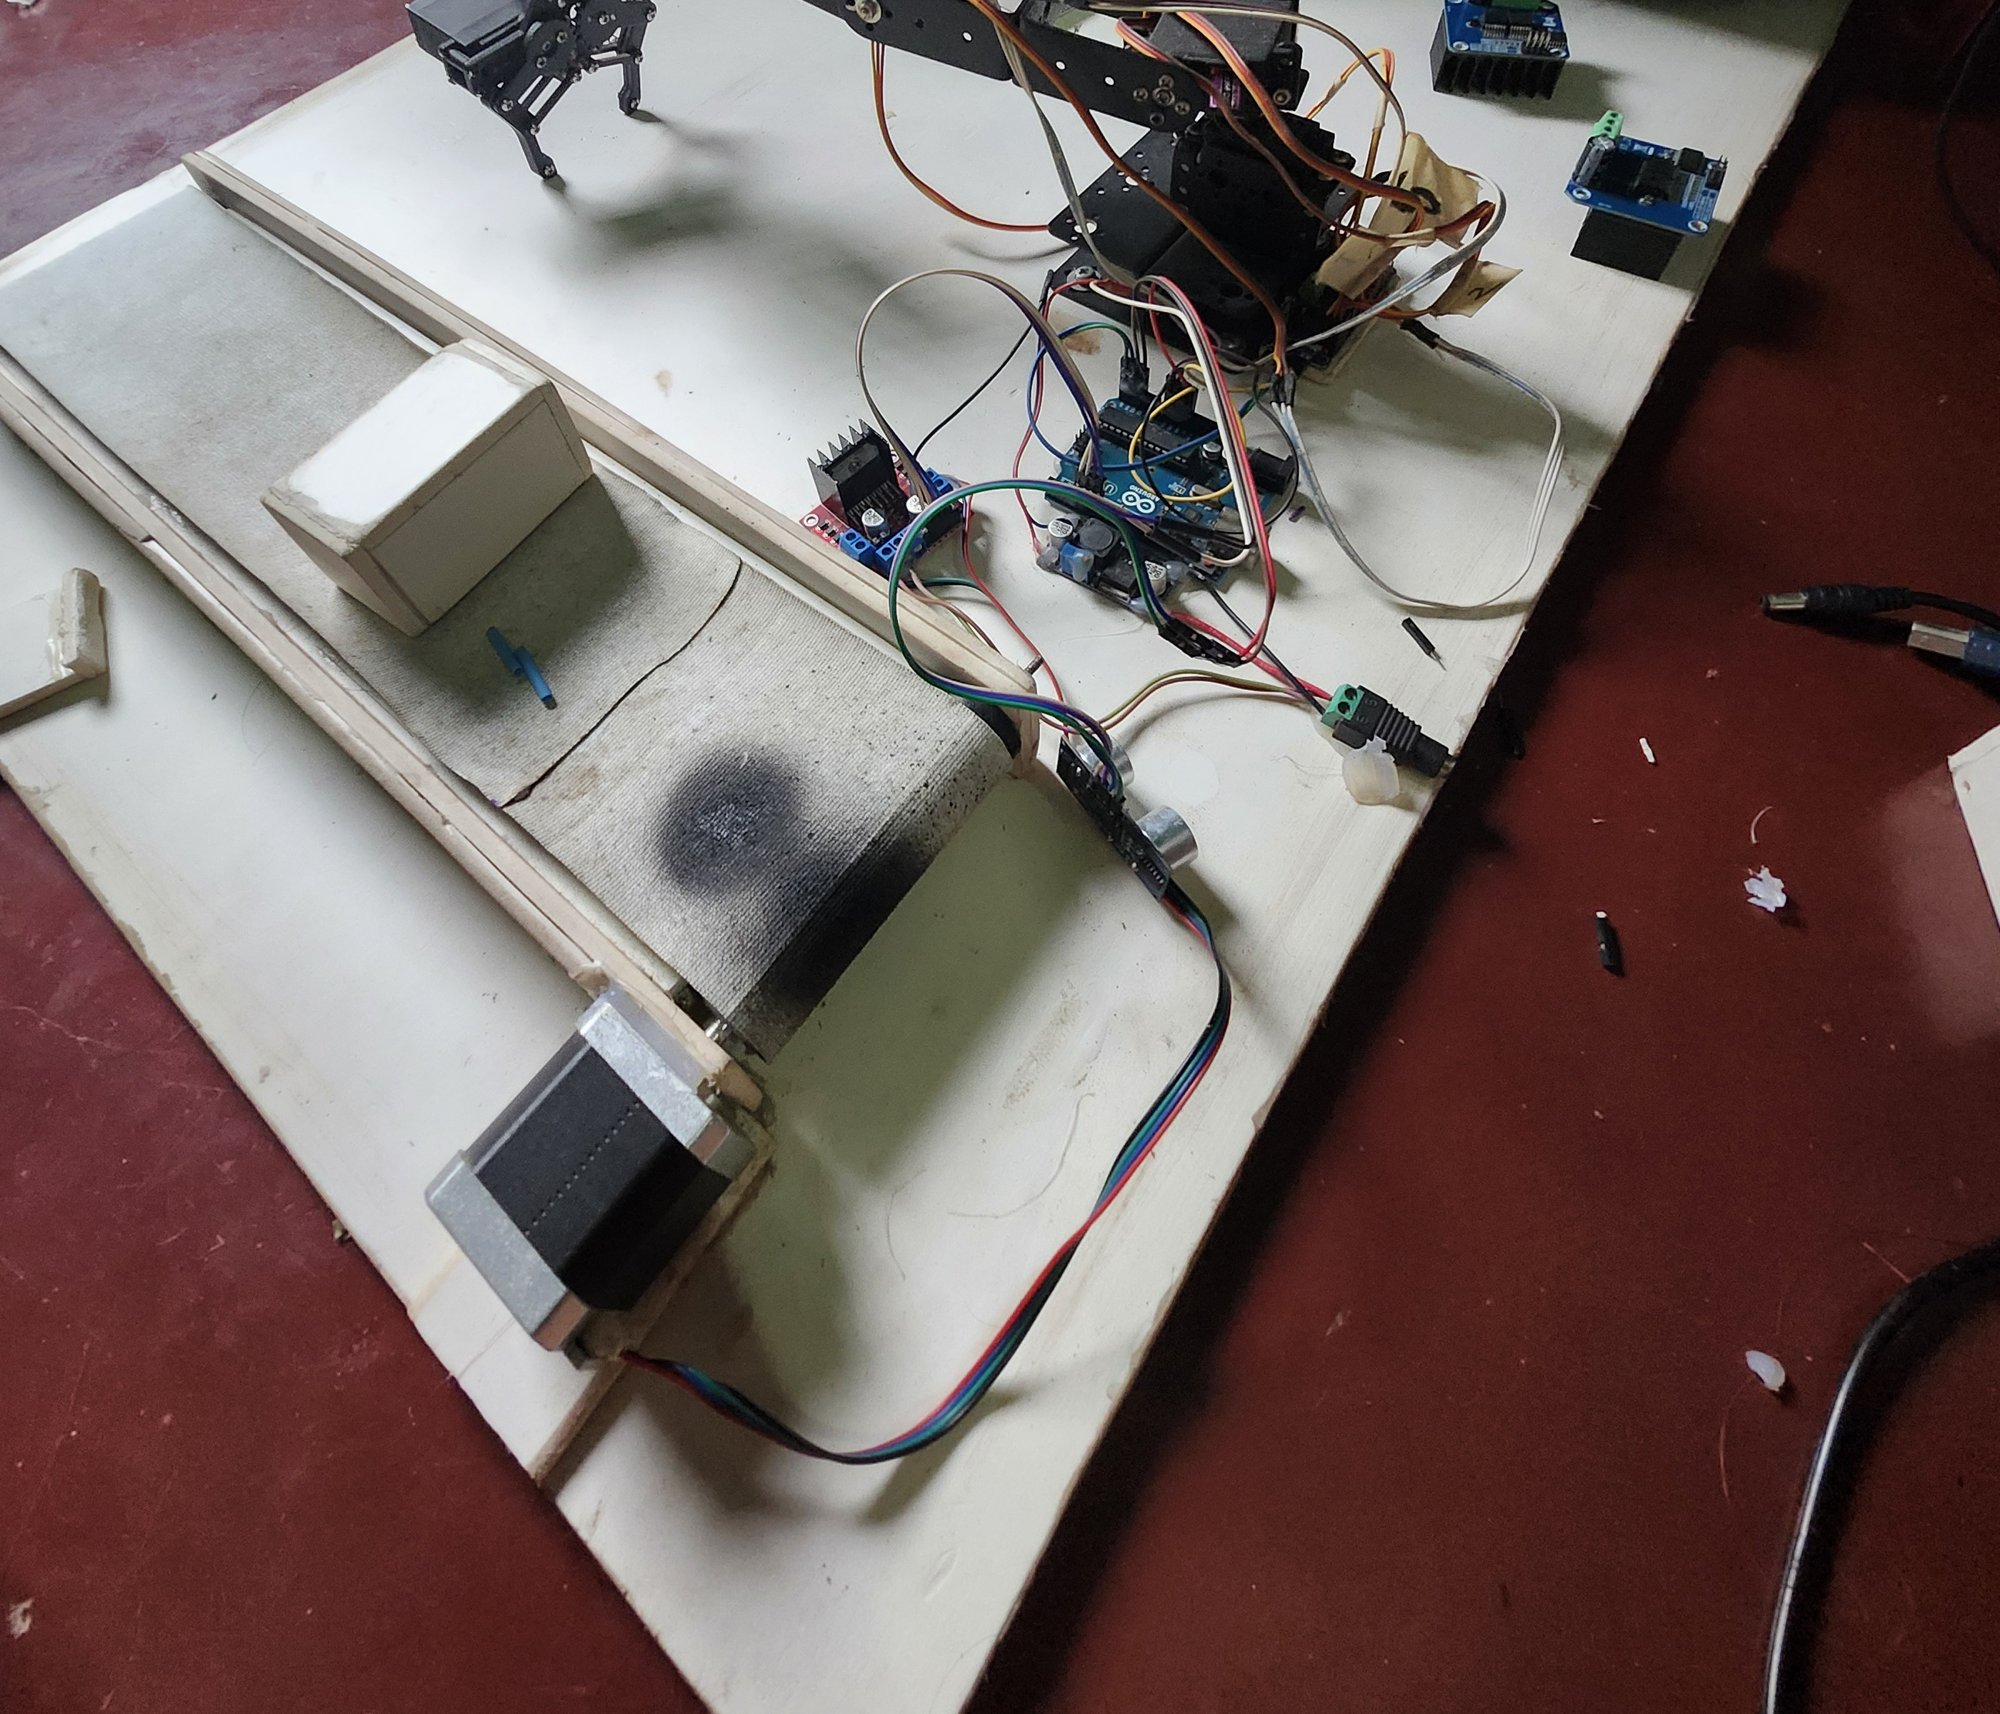
\includegraphics[height=48mm]{conveysort-arm-2024-10-05-arm-on-base.jpg}\hfill
  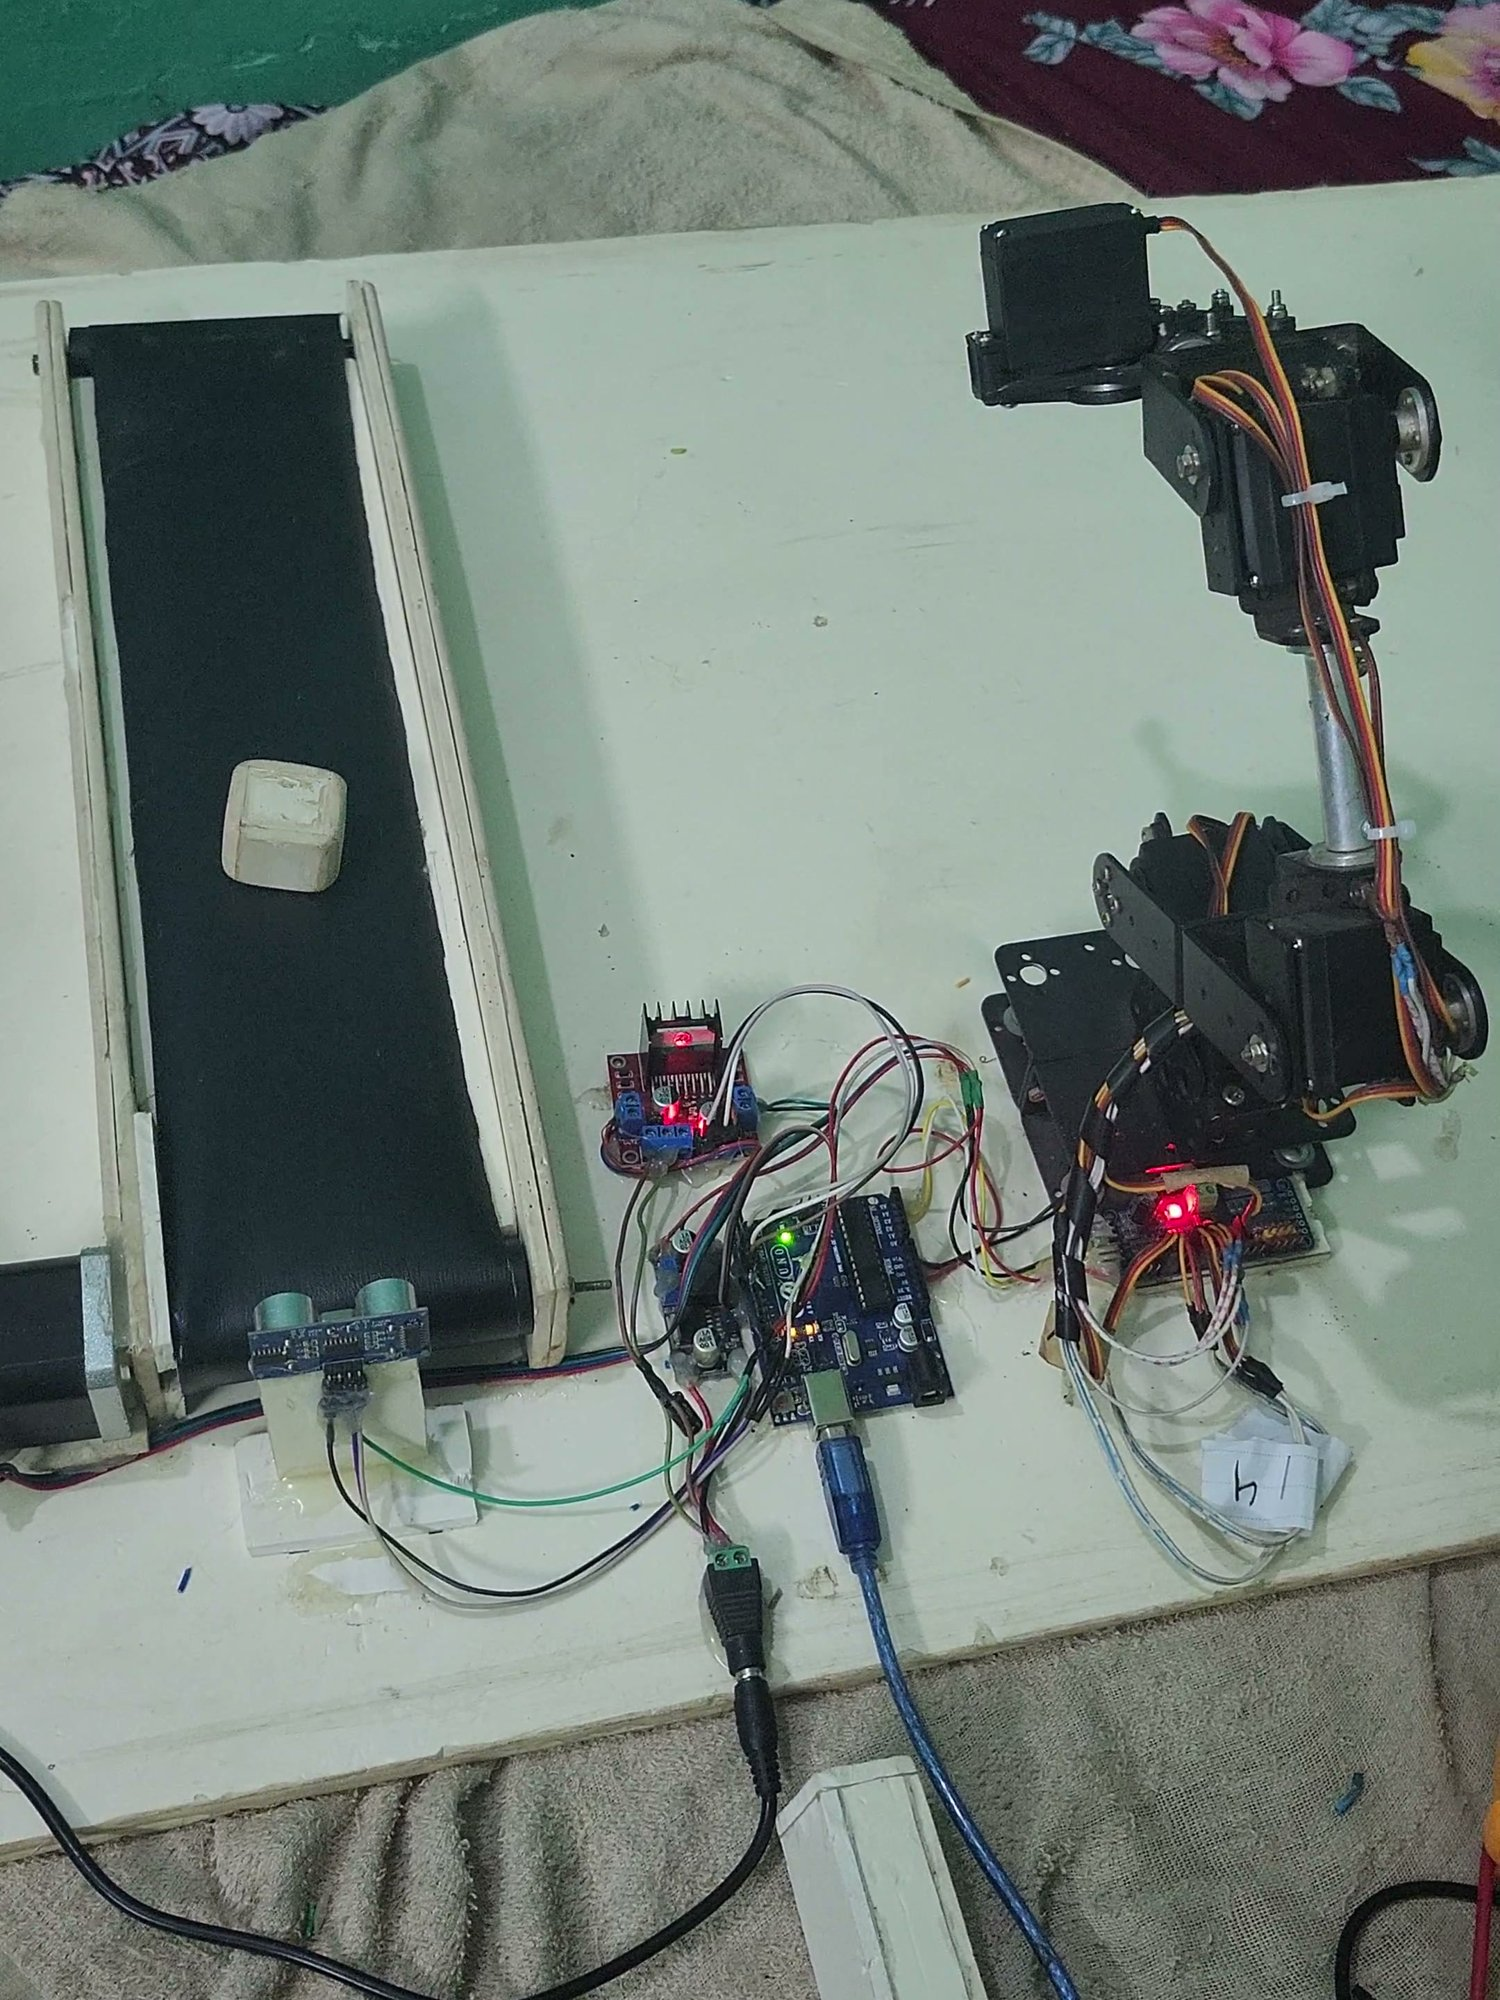
\includegraphics[height=48mm]{conveysort-arm-2024-11-11-belt-and-sensor.jpg}\hfill
  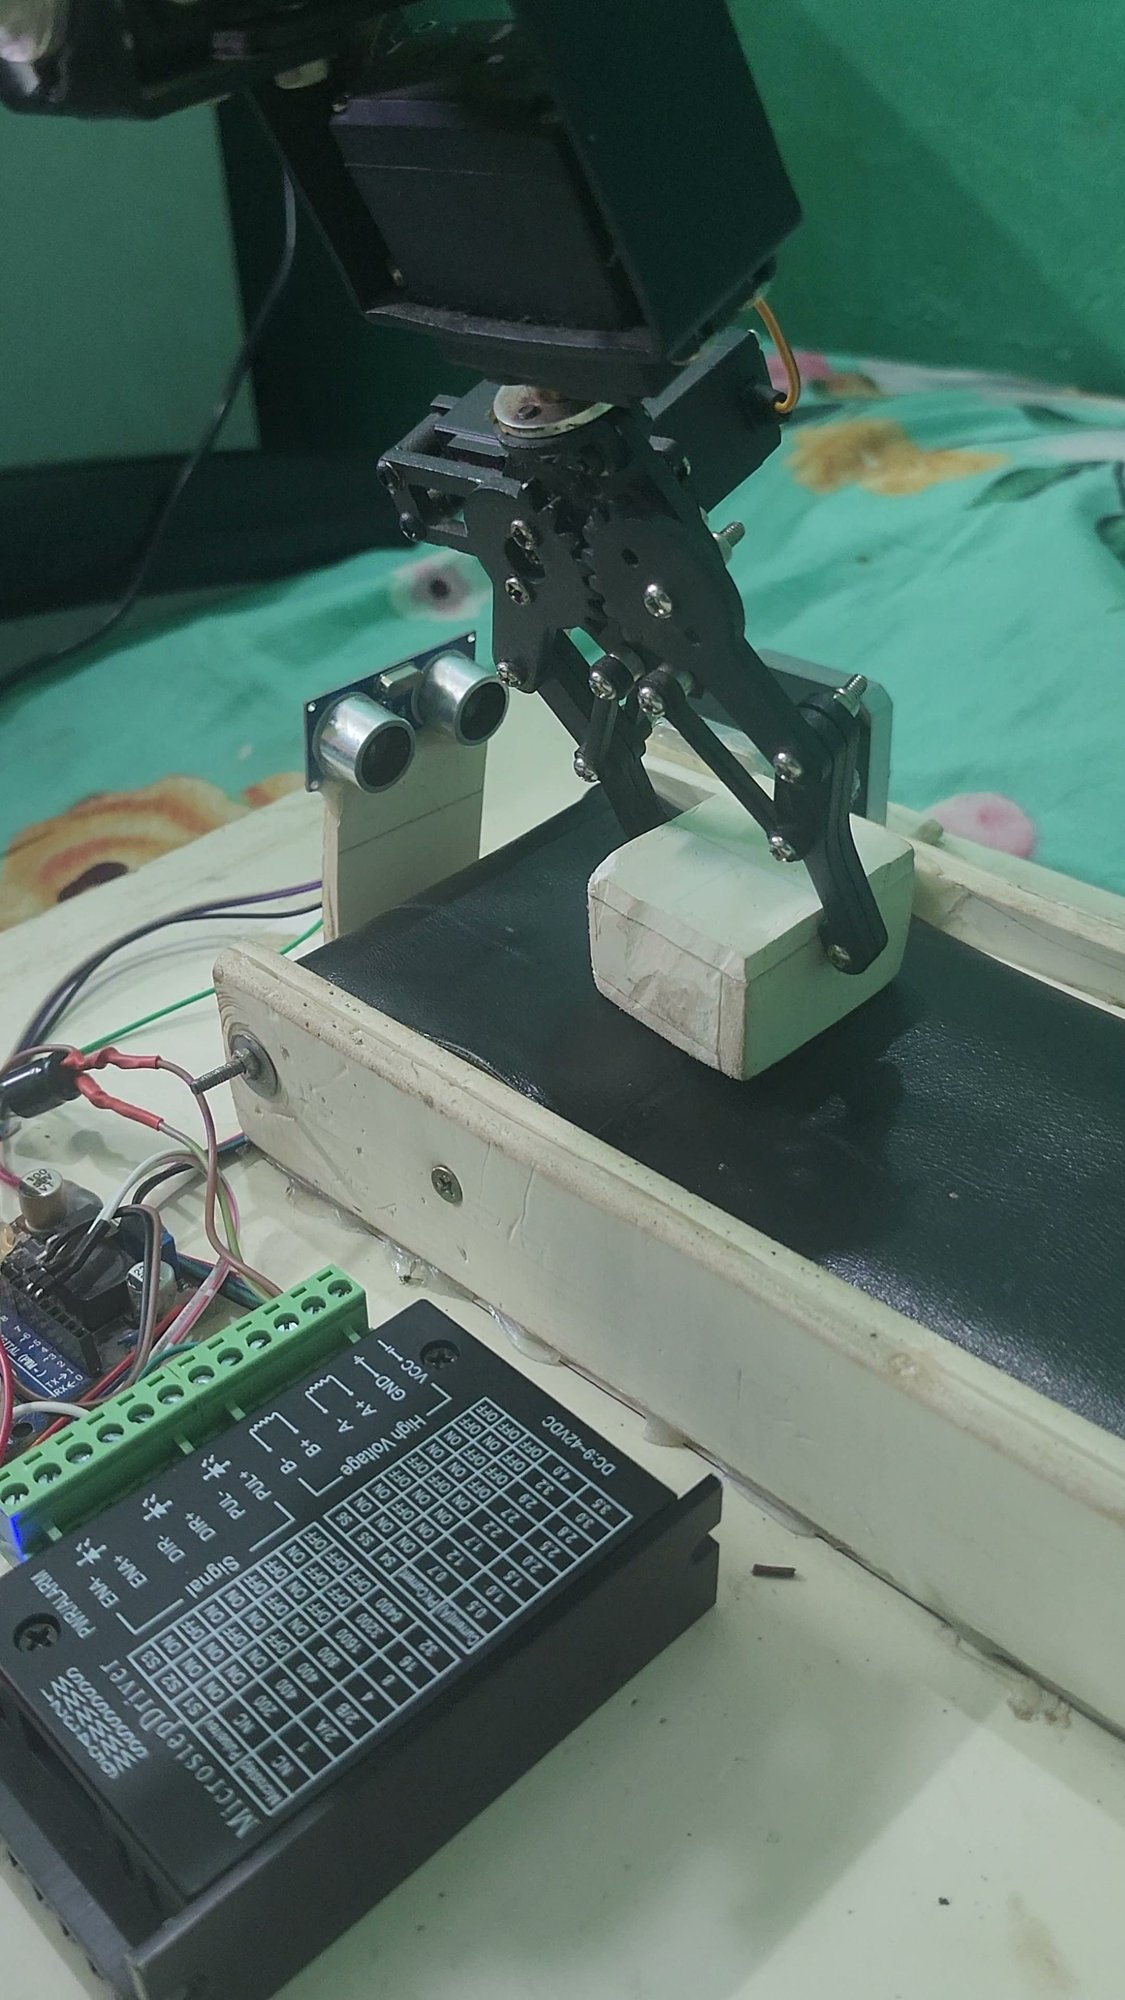
\includegraphics[height=48mm]{conveysort-arm-2024-11-16-gripper-at-sensor.jpg}\hfill
  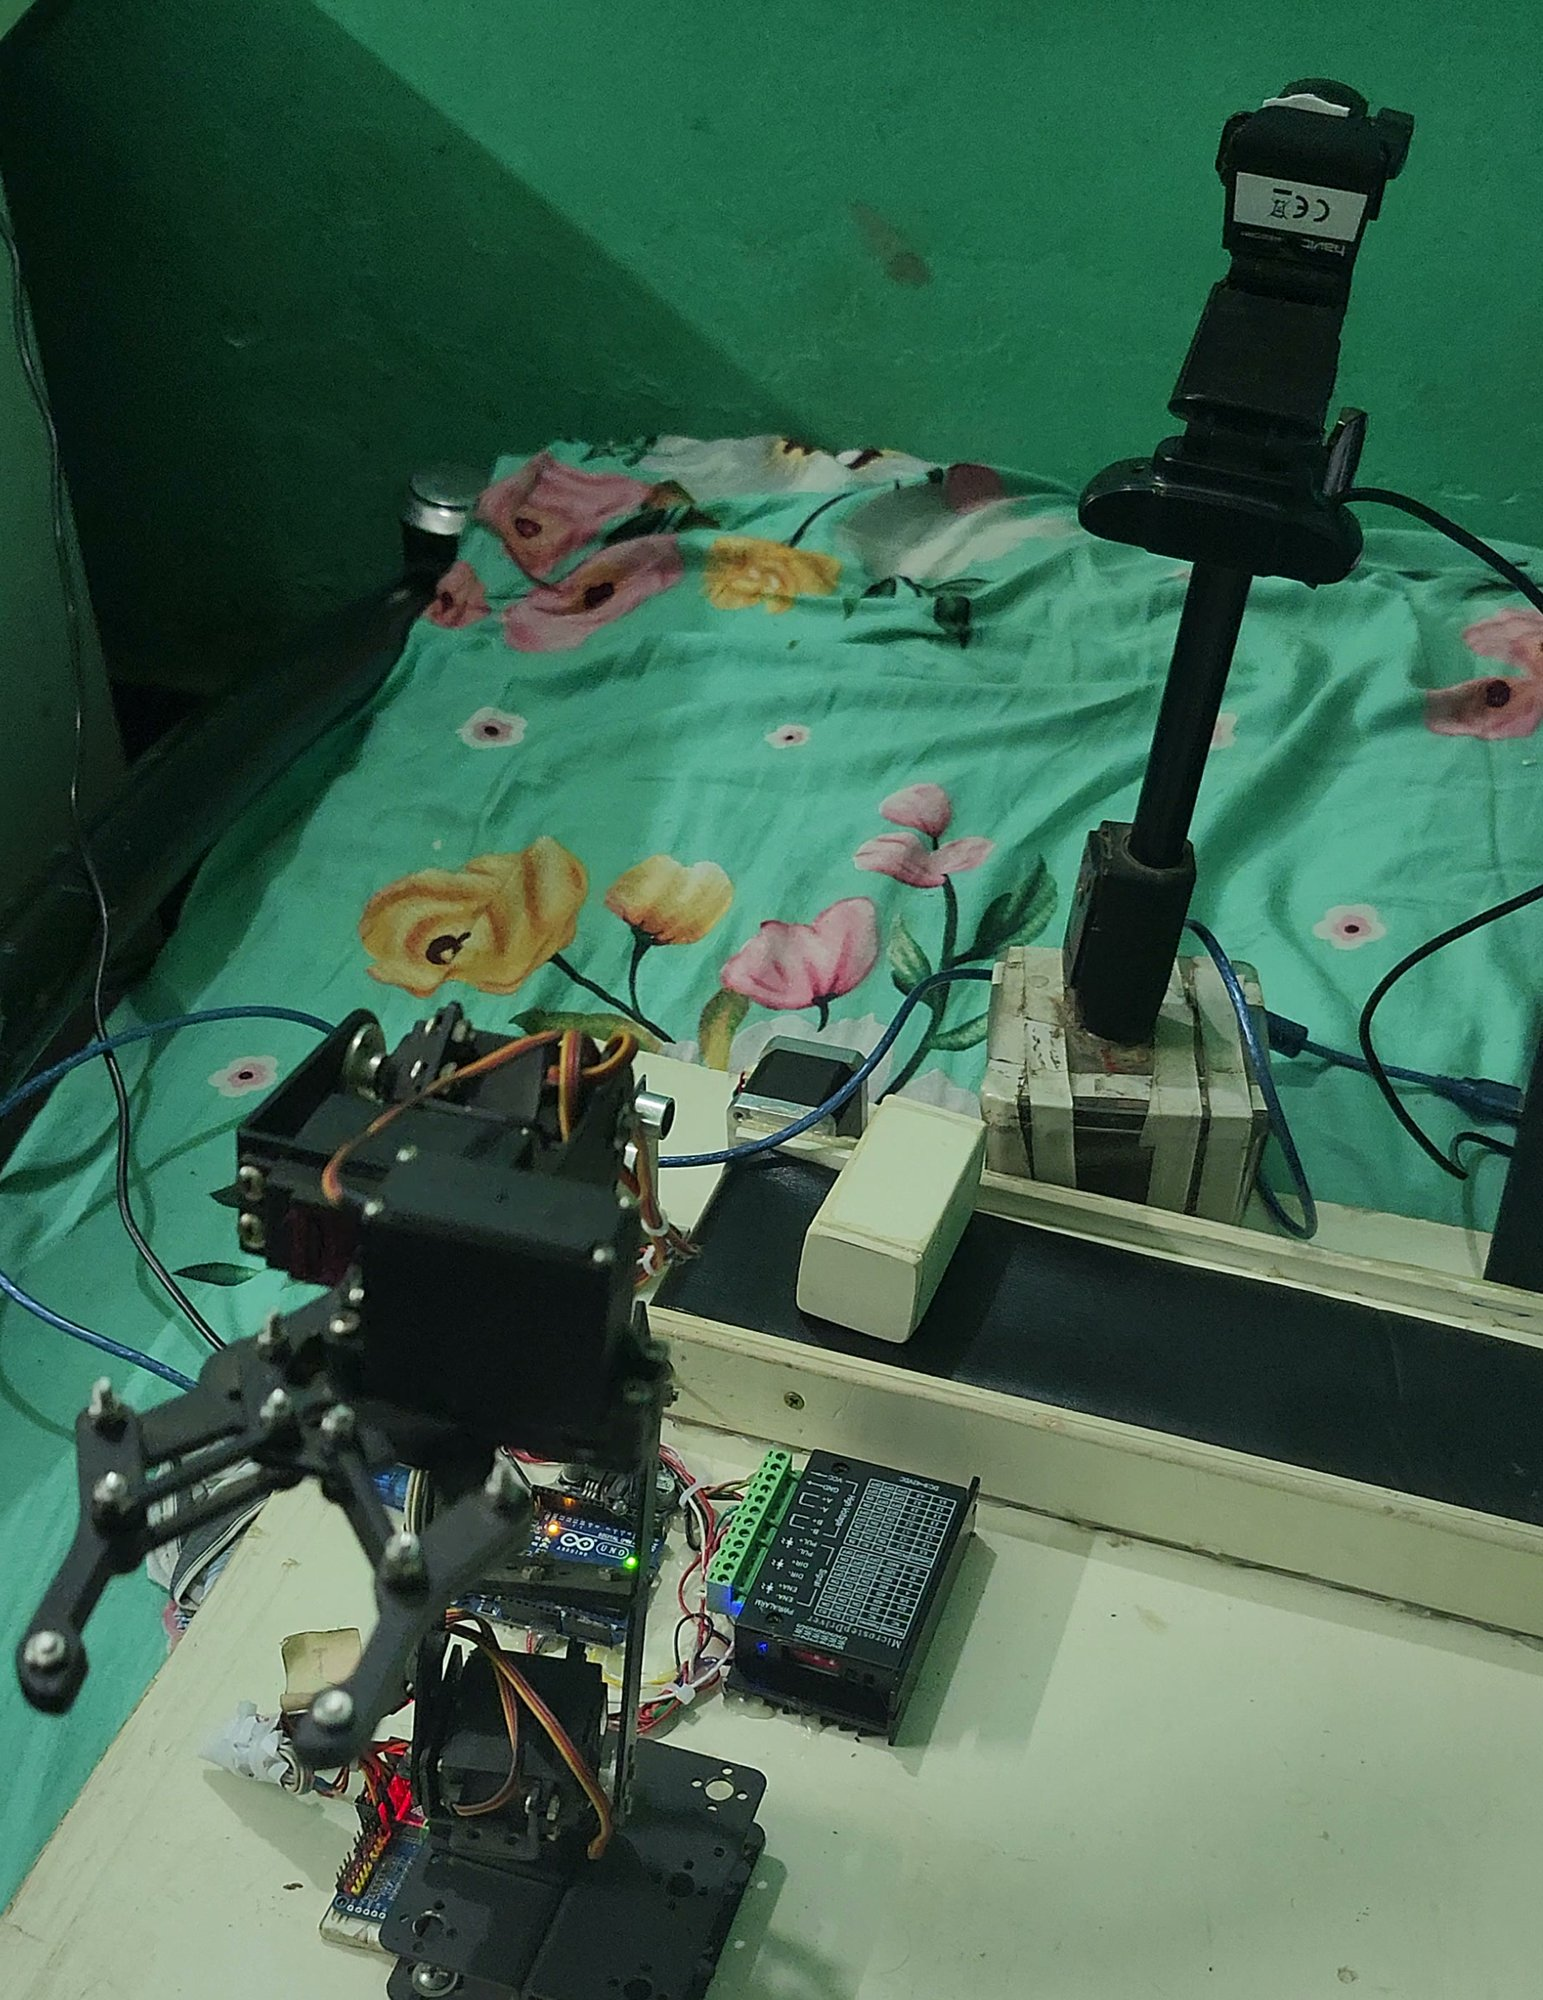
\includegraphics[height=48mm]{conveysort-arm-2024-11-16-camera-on-stand.jpg}
  \caption{The build, in order: the first belt, the sensor, the Arduino and the arm on one board (5 October); the black belt bringing a block to the sensor (11 November); the gripper closing on a block under the sensor, the TB6600 driver in front (16 November); the webcam on its first stand above the belt (16 November).}
  \label{fig:build}
\end{figure}

\begin{figure}[htbp]
  \centering
  \diagramw{0.98}{figures/fig08-timeline}
  \caption{ConveySort-Arm in 2024, from the repository's history and the dated photos and videos.}
  \label{fig:timeline}
\end{figure}

% ---------------------------------------------------------------------------
\section{Electronics}
\label{sec:electronics}

Fig.~\ref{fig:wiring} gives every connection, from the firmware. The stepper driver takes a STEP pulse on pin 5 and a direction on pin 6; the ultrasonic sensor is triggered on pin 9 and answers on pin 8. The PCA9685 sits on the Arduino's I$^2$C pins and drives the six servos at 60\,Hz, on its channels 8, 2, 3, 5, 6 and 7, from the base to the gripper. A servo's angle from 0 to 180$^\circ$ maps to 150--650 of the driver's 4096 counts.

\begin{figure}[htbp]
  \centering
  \diagramw{0.85}{figures/fig02-wiring}
  \caption{The Arduino's connections, from \topic{firmware/conveyor-sorter}: the belt's driver, the sensor, and the servo driver with each joint's channel.}
  \label{fig:wiring}
\end{figure}

% ---------------------------------------------------------------------------
\section{Vision: Sizing a Block}
\label{sec:vision}

\paragraph{From a frame to an outline} The PC reads the webcam at 639 by 480 pixels and mirrors each frame (Fig.~\ref{fig:vision}). It turns the frame grey and keeps a window that leaves out the edges: 100 pixels at the top, 80 at the bottom and 20 at each side, to leave out the image's edges, such as the belt's frame. A 9 by 9 Gaussian blur smooths it, and a threshold at 230 of 255 keeps only the white block on the black belt. OpenCV then finds the outer outlines~\cite{suzuki1985contours}.

\paragraph{Filtering} An outline counts as a block only if its area is at least 1,200 square pixels, both sides of its bounding box are at least 20 pixels, its proportions lie between 1:4 and 4:1, and it lies inside the window. Of the outlines left, the largest is the block.

\begin{figure}[htbp]
  \centering
  \diagramw{0.92}{figures/fig03-vision-pipeline}
  \caption{How the PC sizes a block, from \topic{src/vision/sort_by_size.py}. The threshold and the blur were tuned live with sliders.}
  \label{fig:vision}
\end{figure}

\paragraph{Size by area} The block's size is the area inside its outline (Fig.~\ref{fig:bands}): under 17,000 square pixels it is small, under 28,000 medium, and anything larger is large; that is, under 5.5\% and 9.1\% of the frame. The limits suit the three test blocks with the camera at its working height; they are areas in the image, not sizes in millimetres.

\begin{figure}[htbp]
  \centering
  \diagramw{0.8}{figures/plot01-size-bands}
  \caption{The size classes by outline area. The tuning tool, \topic{object_size_detection.py}, uses 25,000 square pixels for the medium limit; the sorter uses 28,000.}
  \label{fig:bands}
\end{figure}

\paragraph{Deciding} A single frame can be wrong, while a hand passes or the block is still moving. The program therefore counts how many frames in a row give the same size, and sends a size only when ten more frames agree with the first, eleven in a row, and at most once every five seconds (Fig.~\ref{fig:decision}).

\begin{figure}[htbp]
  \centering
  \diagramw{0.5}{figures/fig04-decision-logic}
  \caption{When the PC sends a size: after ten steady frames, and no more than once every five seconds.}
  \label{fig:decision}
\end{figure}

% ---------------------------------------------------------------------------
\section{Control}
\label{sec:control}

\paragraph{The belt} The Arduino reads the ultrasonic sensor every 100\,ms, as the mean of three pings (Fig.~\ref{fig:belt}). With a block 7 to 45\,cm away, it runs the belt; when the block is within 7\,cm, at the belt's end, it stops the belt and reports ``Object detected in position''. Once the block is taken away, the belt waits for the next one. A belt that runs for 30 seconds without a block arriving is reset, and the arm is sent home.

\begin{figure}[htbp]
  \centering
  \diagramw{0.75}{figures/fig05-belt-states}
  \caption{The belt's states, from the distance $d$ the ultrasonic sensor reads.}
  \label{fig:belt}
\end{figure}

\paragraph{The serial protocol} The PC and the Arduino talk in single characters at 9600 baud: \texttt{0} sends the arm home, and \texttt{1}, \texttt{2} and \texttt{3} ask it to sort a small, a medium or a large block (Fig.~\ref{fig:serial}). The Arduino ignores a size, with ``No object detected'', unless the belt has stopped with a block in place, so a size sent early does no harm.

\begin{figure}[htbp]
  \centering
  \diagramw{0.85}{figures/fig06-serial-exchange}
  \caption{One sort, as the messages over the serial link: the Arduino's lines (blue) and the PC's size (orange).}
  \label{fig:serial}
\end{figure}

\paragraph{The pick and place} The arm sorts a block in 15 steps, each moving one joint (Fig.~\ref{fig:pickplace}). It reaches over the belt and down, grips the block, lifts it, turns its base to the block's place, lowers it, and lets go; then it lifts and returns home, joint by joint. Two steps depend on the size: the grip closes to 155$^\circ$, 150$^\circ$ or 140$^\circ$, wider for a larger block, and the base turns to 90$^\circ$, 50$^\circ$ or 10$^\circ$ to set it down in its own place.

\begin{figure}[htbp]
  \centering
  \diagramw{0.98}{figures/fig07-pick-place}
  \caption{The 15-step pick-and-place, from the firmware. Steps 7 and 9 depend on the block's size.}
  \label{fig:pickplace}
\end{figure}

\paragraph{Smooth, safe motion} Each joint moves in steps of 5 counts, about 1.8$^\circ$, every 40\,ms, about 45$^\circ$ per second, and the firmware pauses for a second after each step. After a move, that joint's angle is saved to the Arduino's EEPROM if five seconds have passed since the last save, and at start-up the firmware reads the saved angles back and moves the arm home from them. A watchdog and an error handler send the arm home after a sensor error, a belt time-out or an invalid move.

% ---------------------------------------------------------------------------
\Needspace{10\baselineskip}
\section{Timing}
\label{sec:timing}

Because every move and pause is fixed in the firmware, the time of a sort can be worked out exactly. Replaying the sequence gives the commanded angle of each joint over time (Fig.~\ref{fig:angles}) and the length of each phase (Fig.~\ref{fig:cycle}). One sort, from the command to the arm back home, takes 35.0\,s for a small block, 36.5\,s for a medium one and 37.9\,s for a large one, leaving out the few tenths of a second the bus writes take; the larger blocks go to places further round, so the base turns further. More than half of it, 21\,s, is the one-second pause after each of the 21 moves.

\begin{figure}[htbp]
  \centering
  \diagramw{0.95}{figures/plot02-joint-angles}
  \caption{Commanded joint angles over one sort of a small block, computed from the firmware. The dotted lines mark the phases.}
  \label{fig:angles}
\end{figure}

\begin{figure}[htbp]
  \centering
  \diagramw{0.8}{figures/plot03-cycle-time}
  \caption{The programmed time of one sort, by block size, in its four phases, computed from the firmware.}
  \label{fig:cycle}
\end{figure}

The videos are close to this. In the original 57\,s video of 16 November, read by eye, the gripper is closed on the block by 28\,s and has set it down by 42\,s, about 14\,s later; the firmware gives 13.1\,s from the start of the grip to the end of the release for a small block. The replay is of the code as committed to the repository, in April 2026.

% ---------------------------------------------------------------------------
\Needspace{8\baselineskip}
\section{The ROS~2 Workspace}
\label{sec:ros}

Alongside the sorter, the repository holds a ROS~2 Humble workspace for the arm (Appendix, Fig.~\ref{fig:ros}): its model in URDF, a ros2\_control hardware interface, a MoveIt set-up, launch files for RViz, Gazebo and the real arm, and a task server. It is adapted from Antonio Brandi's course~\cite{brandi2023course}, with the hardware interface, the controllers, the slider node and the arm's sketch changed for six servos in place of four, and the arm's model taken from EnviroBot~\cite{envirobot2026}. Running the arm from it was the team's next step; the project ended first, with the sorter working on its own, so the workspace was written but not run. As written, its task presets still fit the course's arm, and its serial link to the Arduino needs fixing before it can drive this arm.

% ---------------------------------------------------------------------------
\section{Demonstrations}
\label{sec:demo}

The cell's work was recorded on video in November 2024 (Table~\ref{tab:demo}, Fig.~\ref{fig:demo}).

\begin{table}[htbp]
  \centering
  \caption{Behaviours recorded on video.}
  \label{tab:demo}
  \renewcommand{\arraystretch}{1.3}
  \small
  \begin{tabularx}{\textwidth}{@{}>{\sffamily}p{0.13\textwidth}>{\raggedright\arraybackslash}X@{}}
    \toprule
    \thead{Date} & \thead{What the video shows} \\
    \midrule
    11 Nov 2024 & One belt cycle: a block rides the belt to the sensor and stops (original, 51\,s) \\
    16 Nov 2024 & One full cycle before the camera: the belt brings a block, the arm grips it and sets it down (original, 57\,s) \\
    16 Nov 2024 & The tuning window: three blocks placed on the belt in turn by hand, each outlined, measured and called large, medium or small (14\,s) \\
    18 Nov 2024 & The whole cell: the webcam above the belt, the arm taking a block off it, setting it down and going home (original, 178\,s) \\
    \bottomrule
  \end{tabularx}
\end{table}

\begin{figure}[htbp]
  \centering
  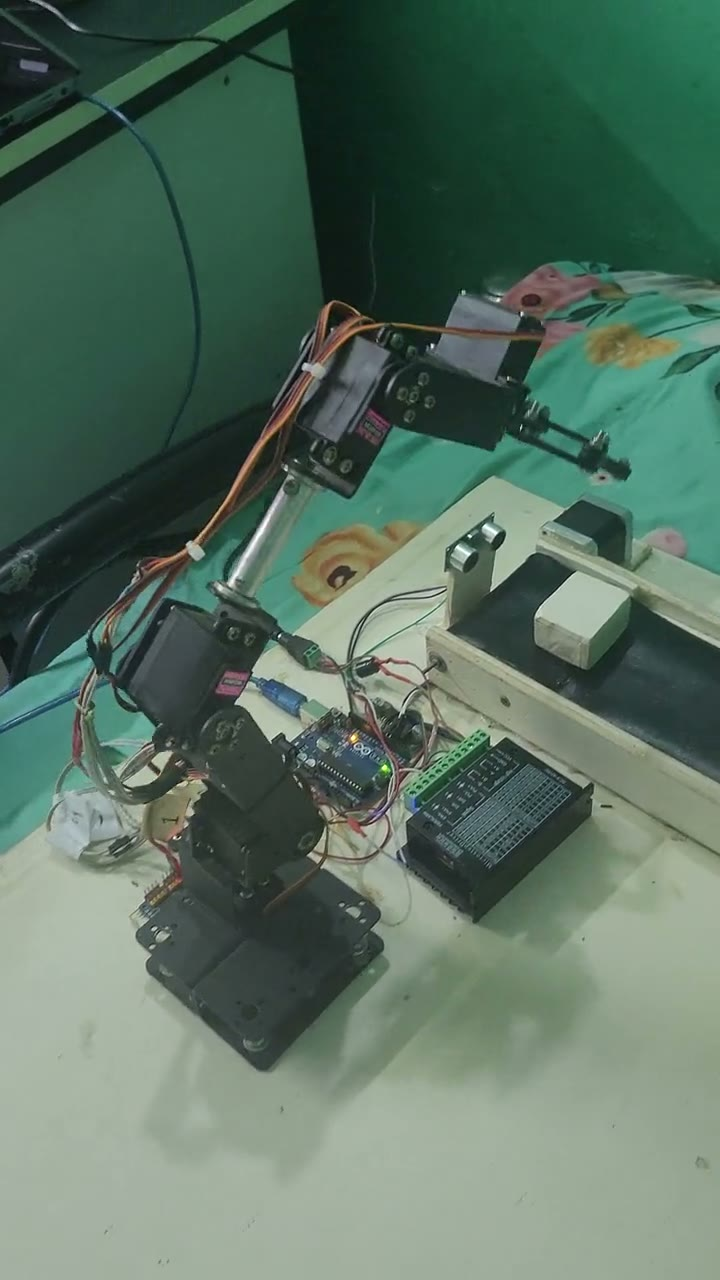
\includegraphics[height=50mm]{conveysort-arm-2024-11-16-belt-sensor-and-arm-poster.jpg}\hfill
  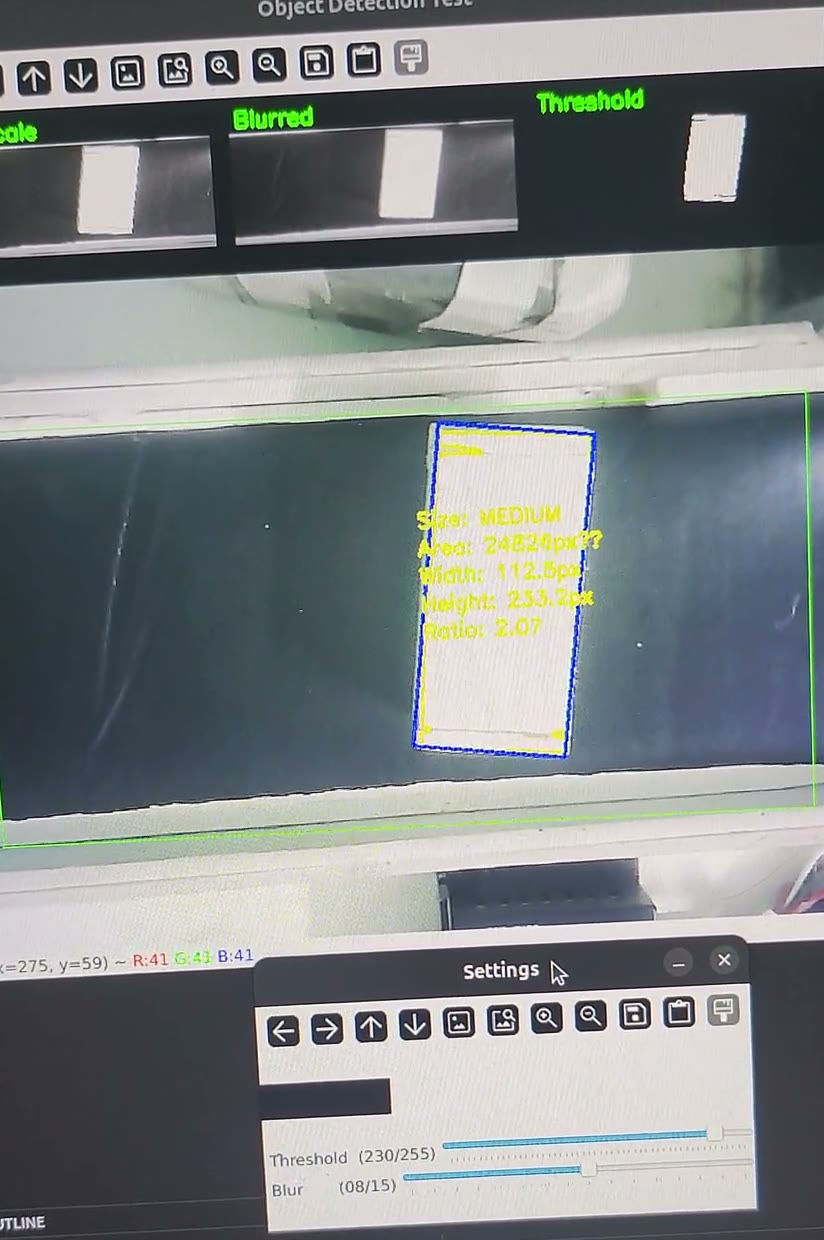
\includegraphics[height=50mm]{conveysort-arm-2024-11-16-camera-detection-poster.jpg}\hfill
  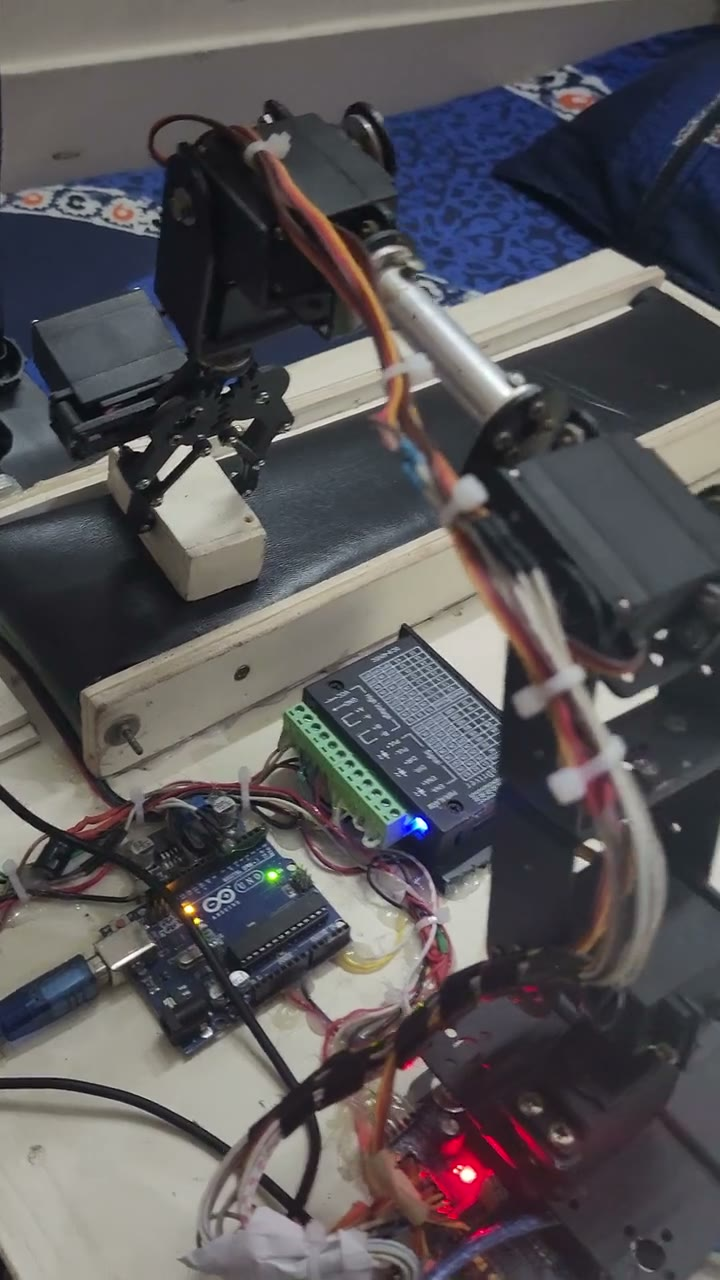
\includegraphics[height=50mm]{conveysort-arm-2024-11-18-arm-camera-and-conveyor-poster.jpg}
  \caption{From the videos: the arm at the end of the belt (16 November); the tuning window outlining and sizing a block (16 November); the whole cell at work (18 November).}
  \label{fig:demo}
\end{figure}

% ---------------------------------------------------------------------------
\section{Lessons Learned}

\paragraph{A physical stop makes picking easy} Stopping each block at the same point, with an ultrasonic sensor, let a fixed sequence pick every block. No grasp planning was needed.

\paragraph{Let each board do what it does well} The PC handled the camera and OpenCV; the Arduino handled timing and motors. One character per sort was all they needed to share.

\paragraph{Steady the decision, not only the image} Waiting for eleven agreeing frames, and acting only when the block is in place, is meant to keep a passing hand or a moving block from triggering a sort, with very little code; the tuning video shows how readily a hand is outlined.

\paragraph{Slow is reliable, but pauses add up} Small steps and a pause after each were chosen to keep the hobby servos steady, at the cost of a sort that takes over half a minute.

% ---------------------------------------------------------------------------
\section{Limitations and Future Work}
\label{sec:future}

ConveySort-Arm was built to work, and its runs were recorded on video rather than counted: its sorting accuracy and its cycle time over many blocks are not yet measured, and its timing here is computed from the firmware. Its sizes are areas in the image, set for one camera height, and its motion is a fixed sequence.

The open steps follow from these (Fig.~\ref{fig:roadmap}): running the arm from the ROS~2 workspace, measuring accuracy and cycle time over many blocks, and calibrating the camera so that sizes are in millimetres; then planning the motion with MoveIt, grasping where the camera sees the block, and sorting by colour and shape as well as size.

\begin{figure}[htbp]
  \centering
  \diagramw{0.98}{figures/fig09-roadmap}
  \caption{What ConveySort-Arm showed in 2024, and the open steps.}
  \label{fig:roadmap}
\end{figure}

% ---------------------------------------------------------------------------
\Needspace{8\baselineskip}
\section{Conclusion}

ConveySort-Arm shows that a working sorting cell can be built from hobby parts and about a thousand lines of code: a belt that stops each block at the arm, a webcam and OpenCV that size it, and a six-servo arm that sets it down in the place for its size. Its split between a PC for vision and an Arduino for motion, joined by one character per sort, keeps each part simple, and its code is open for others to build on.

% ---------------------------------------------------------------------------
\Needspace{10\baselineskip}
\section*{Author Contributions}

Jewel Nath and Shafiul Alam Chowdhury designed, built and tested ConveySort-Arm together at RoboAI. Jewel Nath put its code into its public repository and wrote this report.

\section*{Acknowledgements}

The ROS~2 workspace, three course sketches and the sketch for running the real arm from ROS~2 are adapted from Antonio Brandi's course ``Robotics and ROS~2 -- Learn by Doing! Manipulators'' (Apache~2.0), and each derived file keeps its notice. The ESP32 test sketch comes from Ujwal Nandanwar's RobotArm (MIT), and the development container from the ROS~2 documentation's VS Code guide (CC BY 4.0). The arm's model comes from the first author's earlier EnviroBot project~\cite{envirobot2026}, built at Comilla University with Tasmiara Jahan Toma and Tanjina Akter, where no licence was stated for it; its meshes predate it, and their first source is not known.

This report was written with the help of AI assistants, under the first author's direction; its statements were checked against the code, its history and the dated photos and videos.

{\small
\bibliographystyle{IEEEtran}
\bibliography{references}
}

% ---------------------------------------------------------------------------
\clearpage
\appendix
\section{Additional Material}

\begin{figure}[!ht]
  \centering
  \diagramw{0.8}{figures/fig10-ros2-packages}
  \caption{The ROS~2 Humble workspace, adapted from Antonio Brandi's course: ten packages, written but not run.}
  \label{fig:ros}
\end{figure}

\begin{table}[!ht]
  \centering
  \caption{The repository.}
  \label{tab:repo}
  \renewcommand{\arraystretch}{1.25}
  \small
  \begin{tabularx}{0.92\textwidth}{@{}>{\ttfamily}p{0.3\textwidth}X@{}}
    \toprule
    \thead{Folder} & \thead{Holds} \\
    \midrule
    src/vision/ & the sorter (\topic{sort_by_size.py}) and the tuning tool \\
    firmware/conveyor-sorter/ & the Arduino program for the belt and the arm \\
    src/conveysort\_*/ & the ROS~2 workspace (course-derived, Apache~2.0) \\
    experiments/ & the first belt, sensor and servo tests \\
    docs/media/ & the photos and videos \\
    docs/report/ & this report, its figures and how to build it \\
    docs/diagrams/ & every diagram as its own PDF and PNG \\
    \bottomrule
  \end{tabularx}
\end{table}

\end{document}
